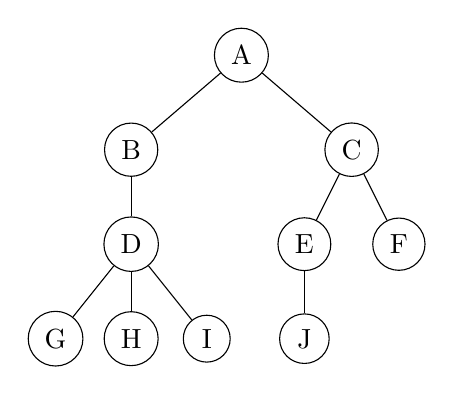
\begin{tikzpicture}[scale=0.8]
  
  %% \tikzstyle{every node}=[ball color=red!70,circle,text=white]
  
  \node [circle,draw] at (0,0) {A}[sibling distance=3.5cm] 
  child { node[circle,draw]{B}
    child {node[circle,draw]{D}[sibling distance=1.2cm]
      child {node[circle,draw]{G}}
      child {node[circle,draw]{H}}
      child {node[circle,draw]{I}}
    }
  }
  child { node[circle,draw]{C}[sibling distance=1.5cm]          
    child {node[circle,draw]{E}
      child {node[circle,draw]{J}} 
    }
    child {node[circle,draw]{F}} 
  };
\end{tikzpicture}
